\subsection*{T9.3}
\subsubsection*{(a)}
\paragraph{}
$p^\star = 1$, with optimal point not attained.
\subsubsection*{(b)}
\begin{figure}[h]
	\centering
	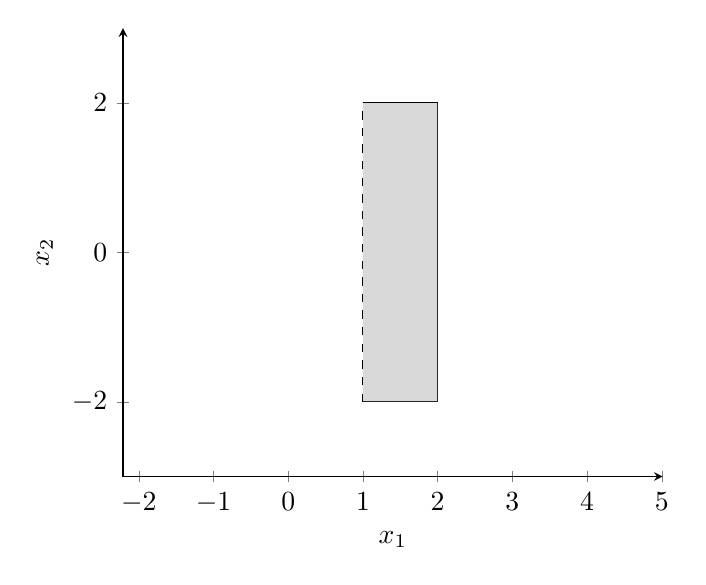
\begin{tikzpicture}
	\begin{axis}[
	axis lines = left,
	xmin=1.3, xmax=1.5, ymin=-3, ymax=3,
	axis equal,
	xlabel = $x_1$,
	ylabel = {$x_2$},
	]
	\addplot[mark=none] coordinates {(1,2) (2,2)};
	\addplot[mark=none] coordinates {(2,-2) (2,2)};
	\addplot[mark=none, dashed] coordinates {(1,-2) (1,2)};
	\addplot[mark=none] coordinates {(1,-2) (2,-2)};
	\fill [gray, opacity=0.3] (axis cs:1,-2) rectangle ( axis cs:2,2);
	\end{axis}
	\end{tikzpicture}
	\caption{Level curve, constraints and feasible set}
\end{figure}
\paragraph{}
The grayed region is the sublevel set. It is not closed since on the boundary $x_1 > 1$. It is strongly convex since there exist $m \geq 0 $, for instance, $m=1$, such that the \textit{Hessian}
\begin{align*}
\triangledown^2f(x) = 2I \succeq mI
\end{align*}
\subsubsection*{(c)}
\paragraph{}
No, since it requires the sublevel set $S$ to be closed.